\section{実行結果}

\subsection{実行環境}

プログラムは以下の環境で実行した。実行出力の全文は付録 B に無加工で示す。

\begin{table}[htbp]
\centering
\caption{実行環境}
\label{tab:env}
\begin{tabular}{ll}
\hline
項目 & 内容 \\
\hline
OS & macOS (Darwin 25.5.0) \\
Python & 3.13.2 \\
OpenCV ({\tt cv2}) & 4.12.0 \\
numpy & 2.4.4 \\
matplotlib & 3.10.6 \\
scipy & 1.15.2 \\
\hline
\end{tabular}
\end{table}

データセットのパスは、課題指定の Colab パスを既定値とし、手元環境では環境変数
{\tt DATASET\_ROOT} で差し替えて実行した(プログラムの変更はない)。

\subsection{課題 1: 動画の読み込み}

People - 84973.mp4 について、横 1280、縦 720、FPS 25.0、総フレーム数 241 が
出力された。1280$\times$720 は HD 解像度であり、再生時間は $241 / 25.0 = 9.64$ 秒に
相当する。

\subsection{課題 2: サムネイル画像の作成}

代表フレームとしてフレーム 185 が選択され、図 \ref{fig:thumbnail} のサムネイルが
保存された。人物が画面中央付近に大きく写っており、動画の内容を代表する画像が
得られている。

\begin{figure}[htbp]
\centering
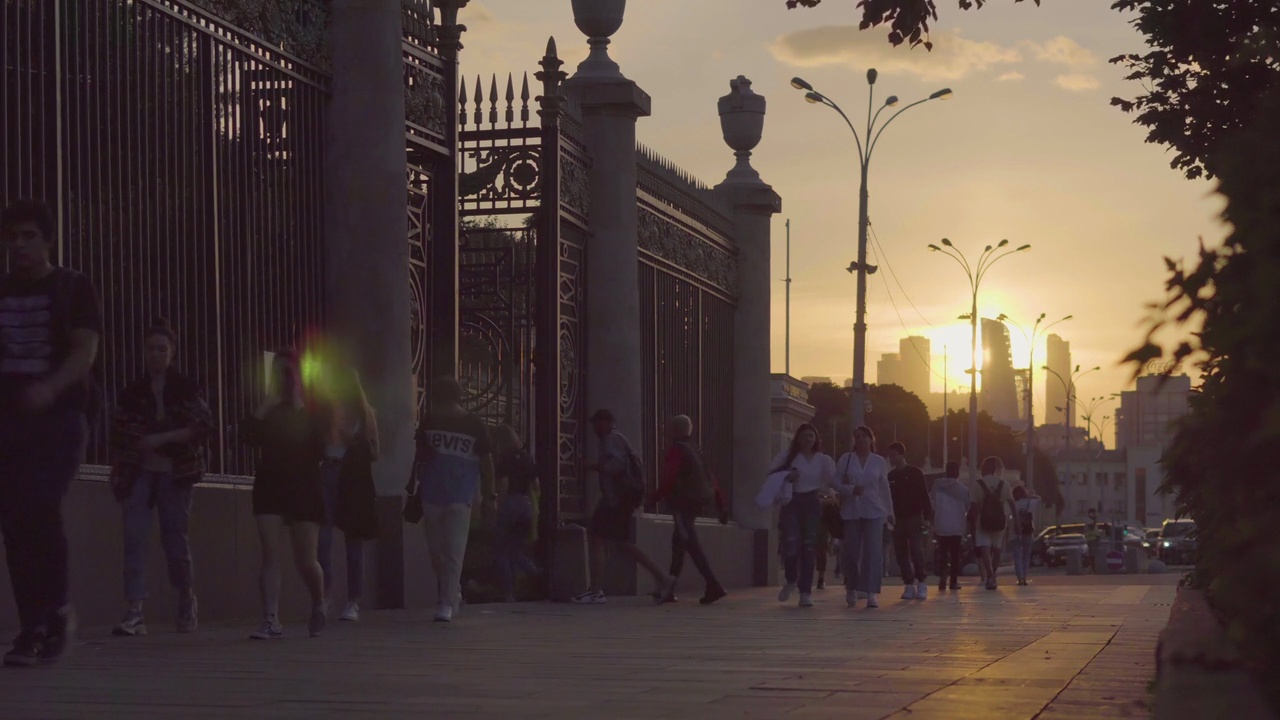
\includegraphics[width=0.7\linewidth]{../dataset/images/output/6324034_thumbnail.jpg}
\caption{選択されたサムネイル画像(フレーム 185)}
\label{fig:thumbnail}
\end{figure}

\subsection{課題 3: ファイル名のパース}

「People - 84973.mp4」に対して Title: People、ID: 84973 が、
「Cat - 66004.mp4」に対して Title: Cat、ID: 66004 が出力され、
いずれも課題の出力結果例と一致した。

\subsection{課題 4: 色反転と動画の保存}

Cat - 66004.mp4(1280$\times$720、294 フレーム)から、色反転した
384$\times$216 の動画 6324034\_cat\_reverse.mp4 が保存された。
出力サイズは $1280 \times 0.3 = 384$、$720 \times 0.3 = 216$ であり、
指定どおり縦・横それぞれ 0.3 倍になっている。

\subsection{課題 5: 音声の可視化}

report\_audio.wav(標本化周波数 44100 Hz、264600 サンプル、約 6.0 秒)の
スペクトログラムを図 \ref{fig:spectrogram} に示す。窓長 1024、オーバーラップ 768、
ハン窓、dB 表示の設定で、時間-周波数領域に隠されたメッセージ
「Good work」が判読できた。

\begin{figure}[htbp]
\centering
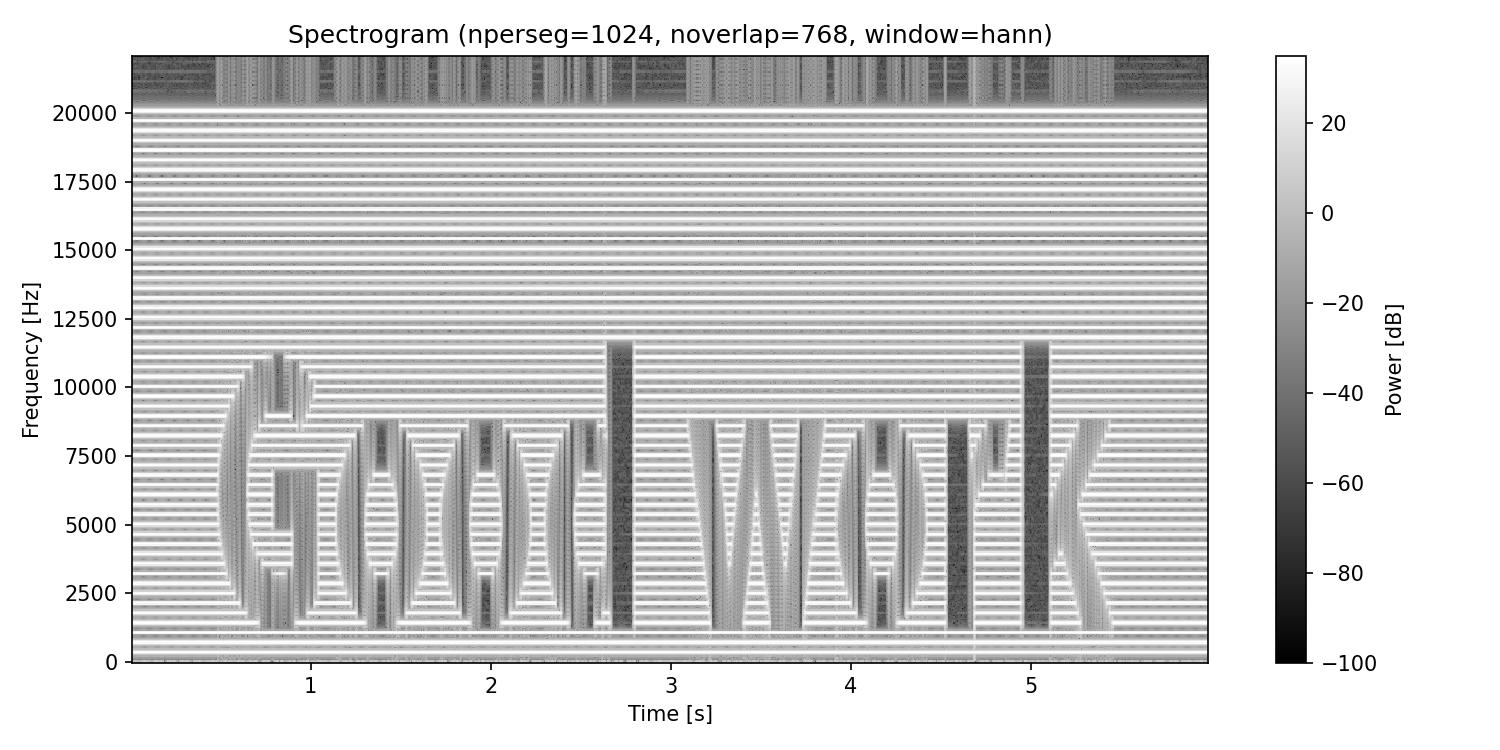
\includegraphics[width=0.95\linewidth]{../dataset/images/output/6324034_spectrogram.jpg}
\caption{report\_audio.wav のスペクトログラム(窓長 1024、オーバーラップ 768、ハン窓)}
\label{fig:spectrogram}
\end{figure}

\subsection{課題 6: n-gram}

stop words を除去しない場合(6-a)の上位 10 個の 2-gram を図 \ref{fig:2gram} に、
stop words を除去した場合(6-b)を図 \ref{fig:2gram_sw} に示す。
テキストの総単語数は 984、stop words 除去後は 614 であった。
除去前の 1 位は「natural language」(15 回)で、「in the」「of the」などの
機能語の組が上位に混在した。除去後は「natural language」「language processing」
「machine translation」など内容語の組のみが上位を占めた。

\begin{figure}[htbp]
\centering
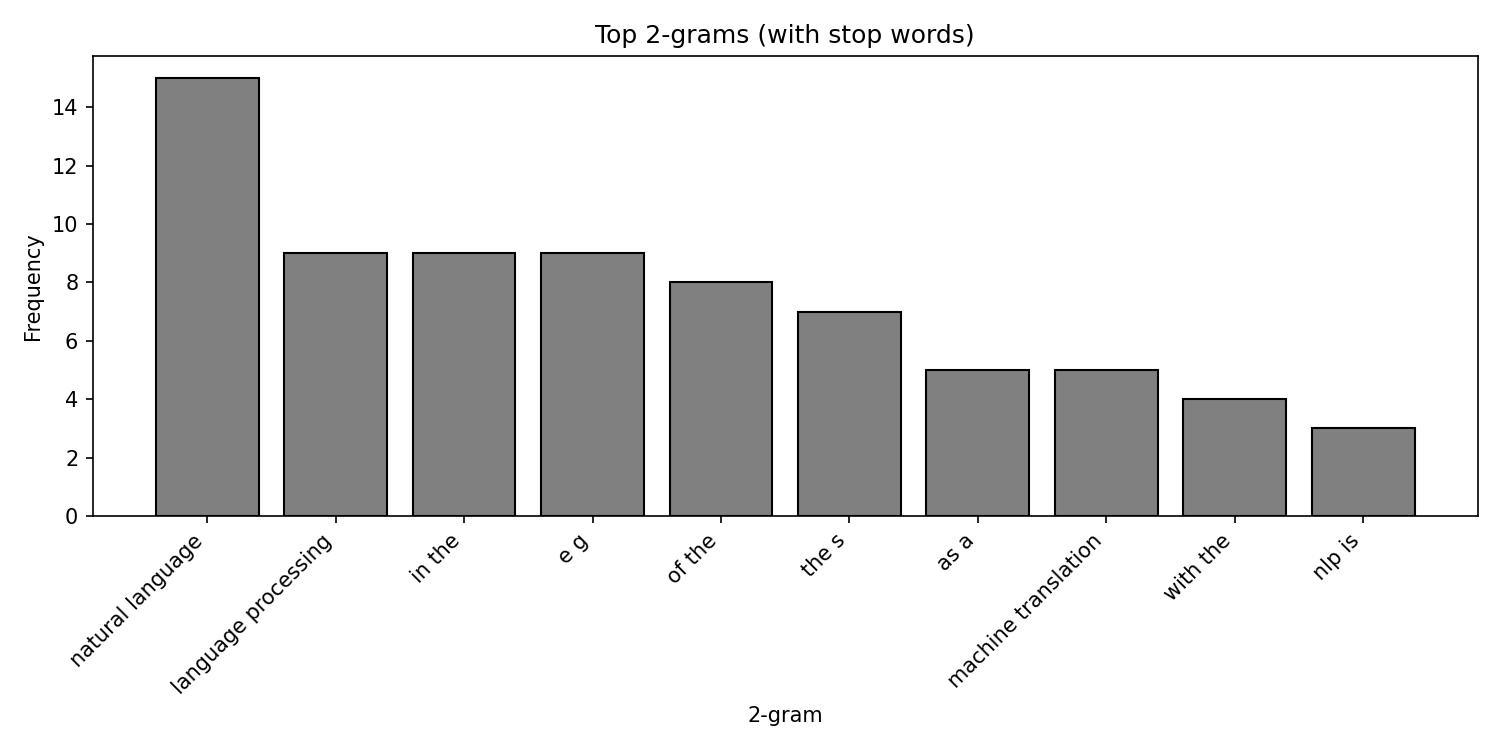
\includegraphics[width=0.9\linewidth]{../dataset/images/output/6324034_2gram_graph.jpg}
\caption{2-gram 出現頻度上位 10 個(stop words 除去なし)}
\label{fig:2gram}
\end{figure}

\begin{figure}[htbp]
\centering
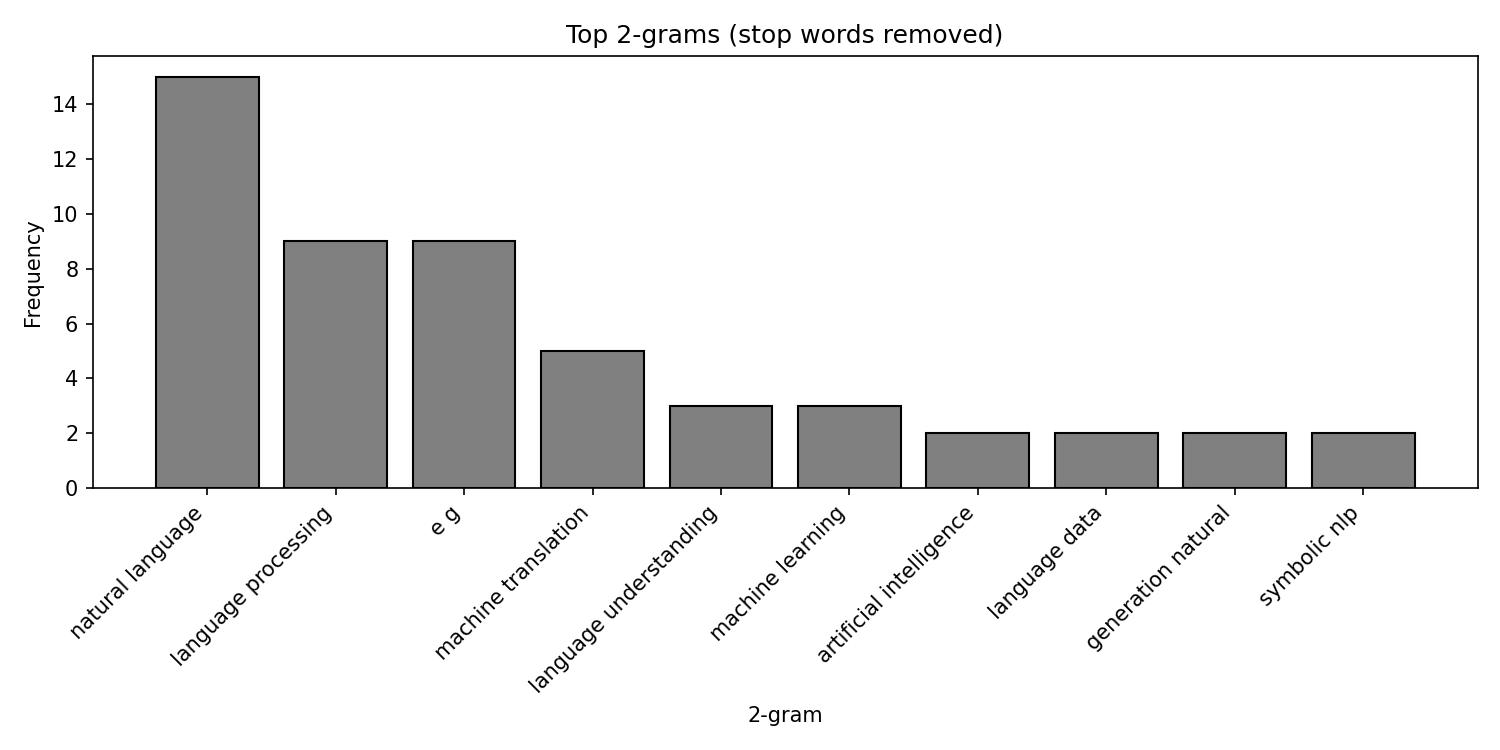
\includegraphics[width=0.9\linewidth]{../dataset/images/output/6324034_2gram_graph_no_stopwords.jpg}
\caption{2-gram 出現頻度上位 10 個(stop words 除去あり)}
\label{fig:2gram_sw}
\end{figure}

\subsection{課題 7: 動画の変わり目検出}

Detection.mp4 は 322 フレームからなり、隣接フレーム間の変化量は 321 個
計算された。変化量の推移を図 \ref{fig:framediff} に示す。3 本の突出した
ピークが確認できる。

\begin{figure}[htbp]
\centering
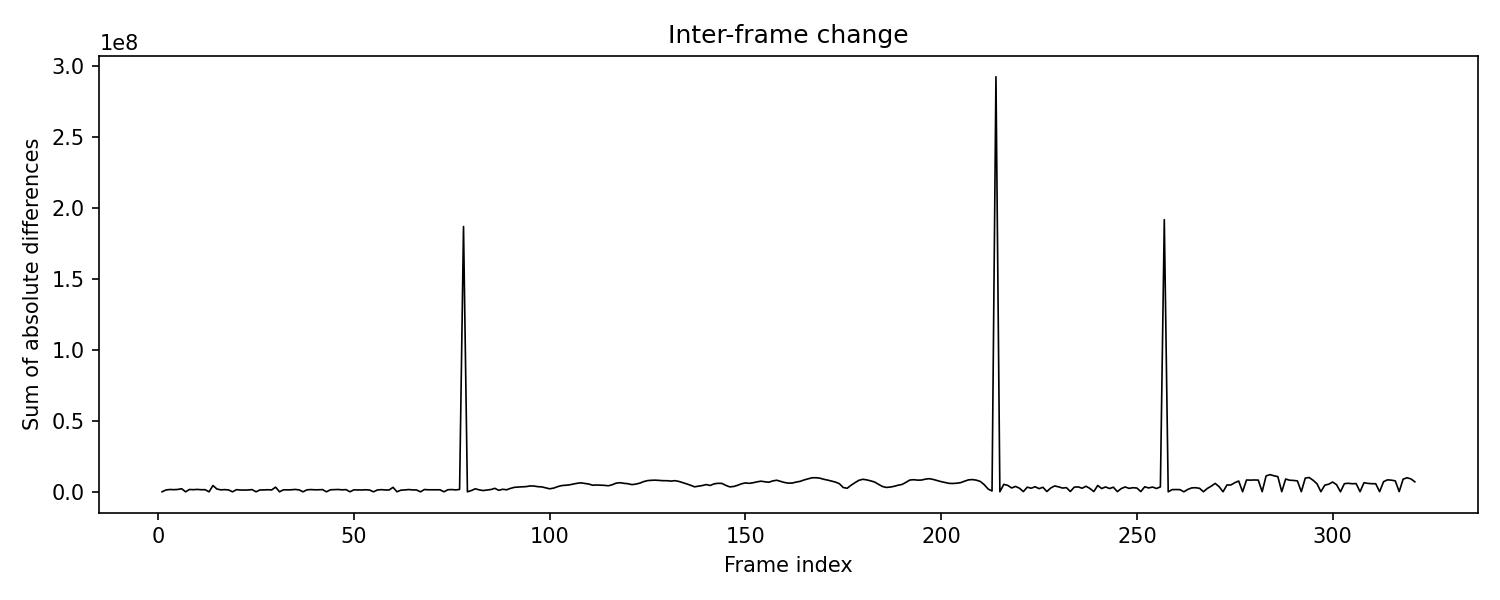
\includegraphics[width=0.95\linewidth]{../dataset/images/output/6324034_framediff.jpg}
\caption{隣接フレーム間の画素値変化量の推移}
\label{fig:framediff}
\end{figure}

3 方式の検出結果を表 \ref{tab:detect} に示す。いずれの方式でも
フレーム 78、214、257 が変わり目として検出され、結果は一致した。

\begin{table}[htbp]
\centering
\caption{閾値決定方式ごとの変わり目検出結果}
\label{tab:detect}
\begin{tabular}{lll}
\hline
方式 & 閾値・条件 & 検出フレーム \\
\hline
平均 $+3\sigma$ & $\theta = 71682248.1$ & 78, 214, 257 \\
上位 3 ピーク & 変化量降順 3 個 & 78, 214, 257 \\
移動平均基準 & 窓 15、係数 4.0 & 78, 214, 257 \\
\hline
\end{tabular}
\end{table}

検出されたフレームとその直前フレームの画像を図 \ref{fig:boundary} に示す。
いずれの箇所でも直前フレームと検出フレームで場面が完全に入れ替わっており、
検出された 3 フレームが実際に動画の変わり目であることが確認できた。

\begin{figure}[htbp]
\centering
\begin{tabular}{cc}
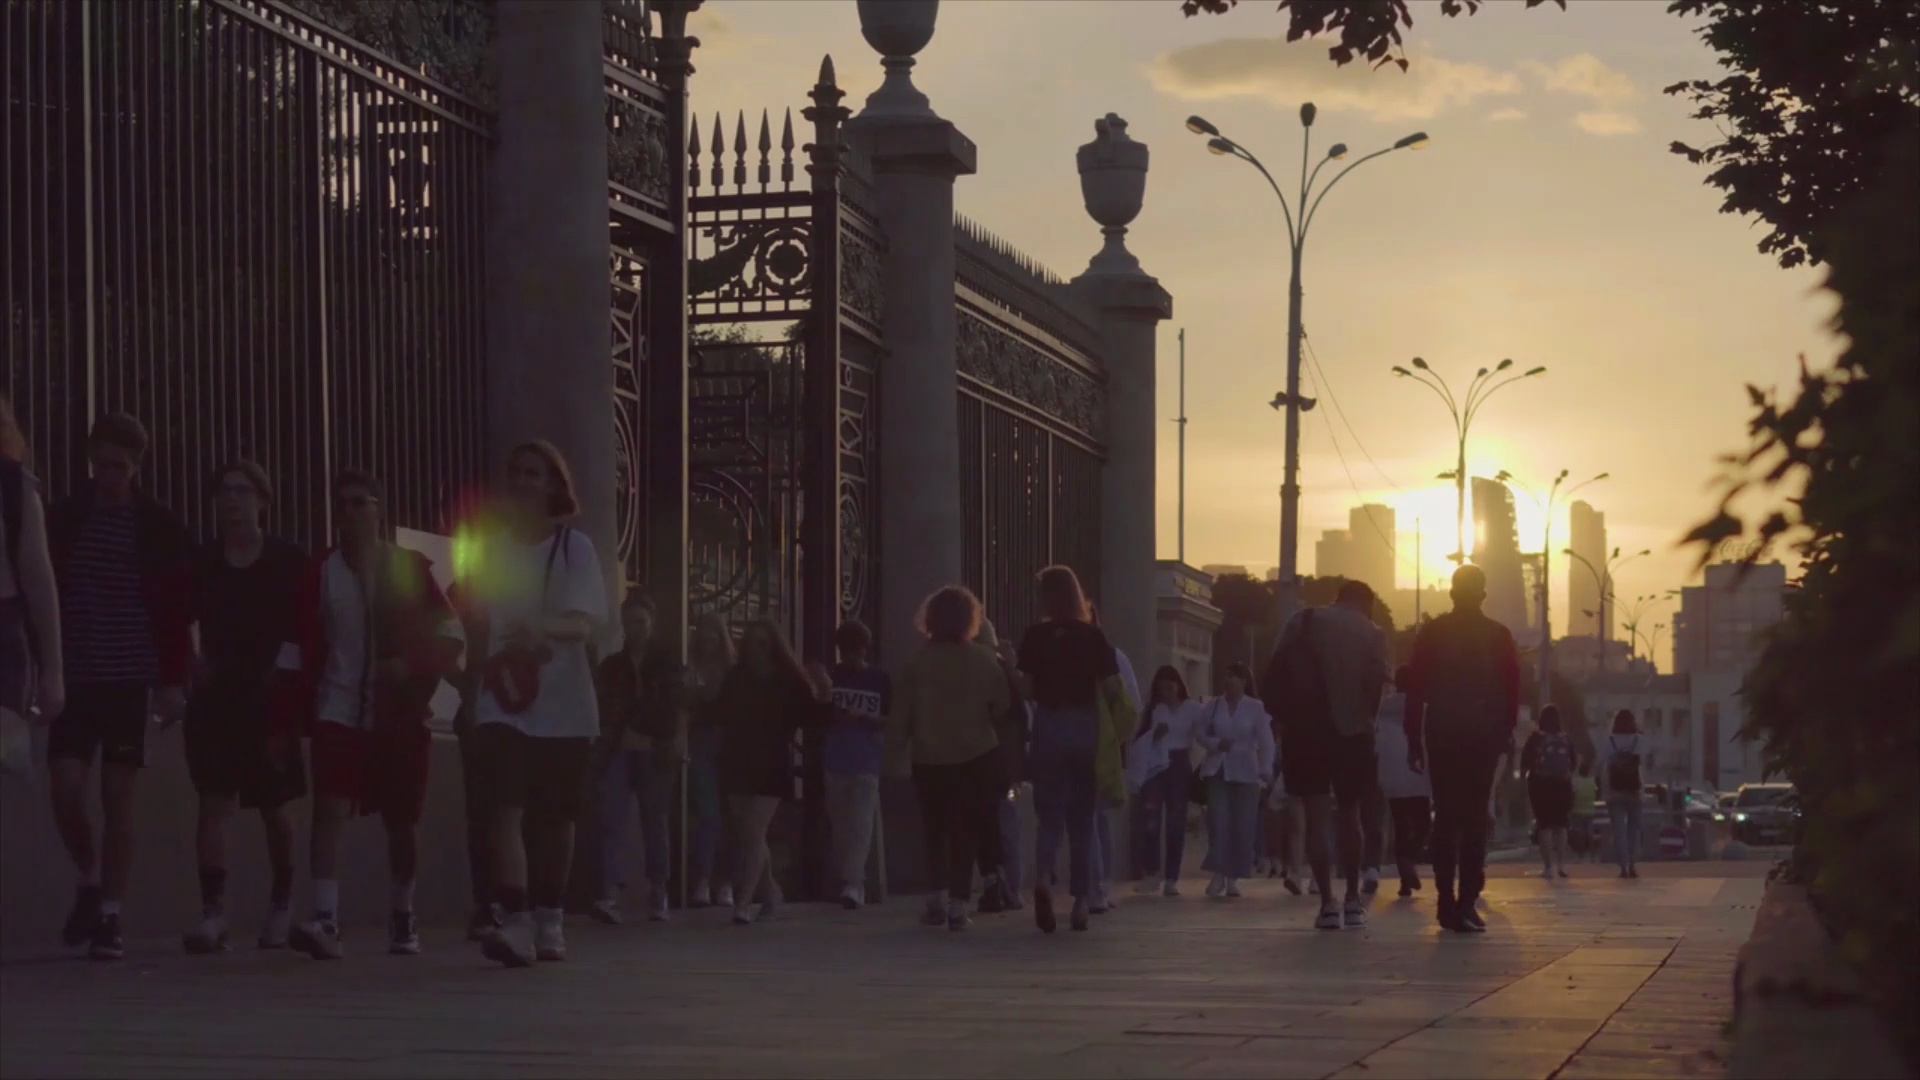
\includegraphics[width=0.42\linewidth]{../dataset/images/output/6324034_boundary_frame77.jpg} &
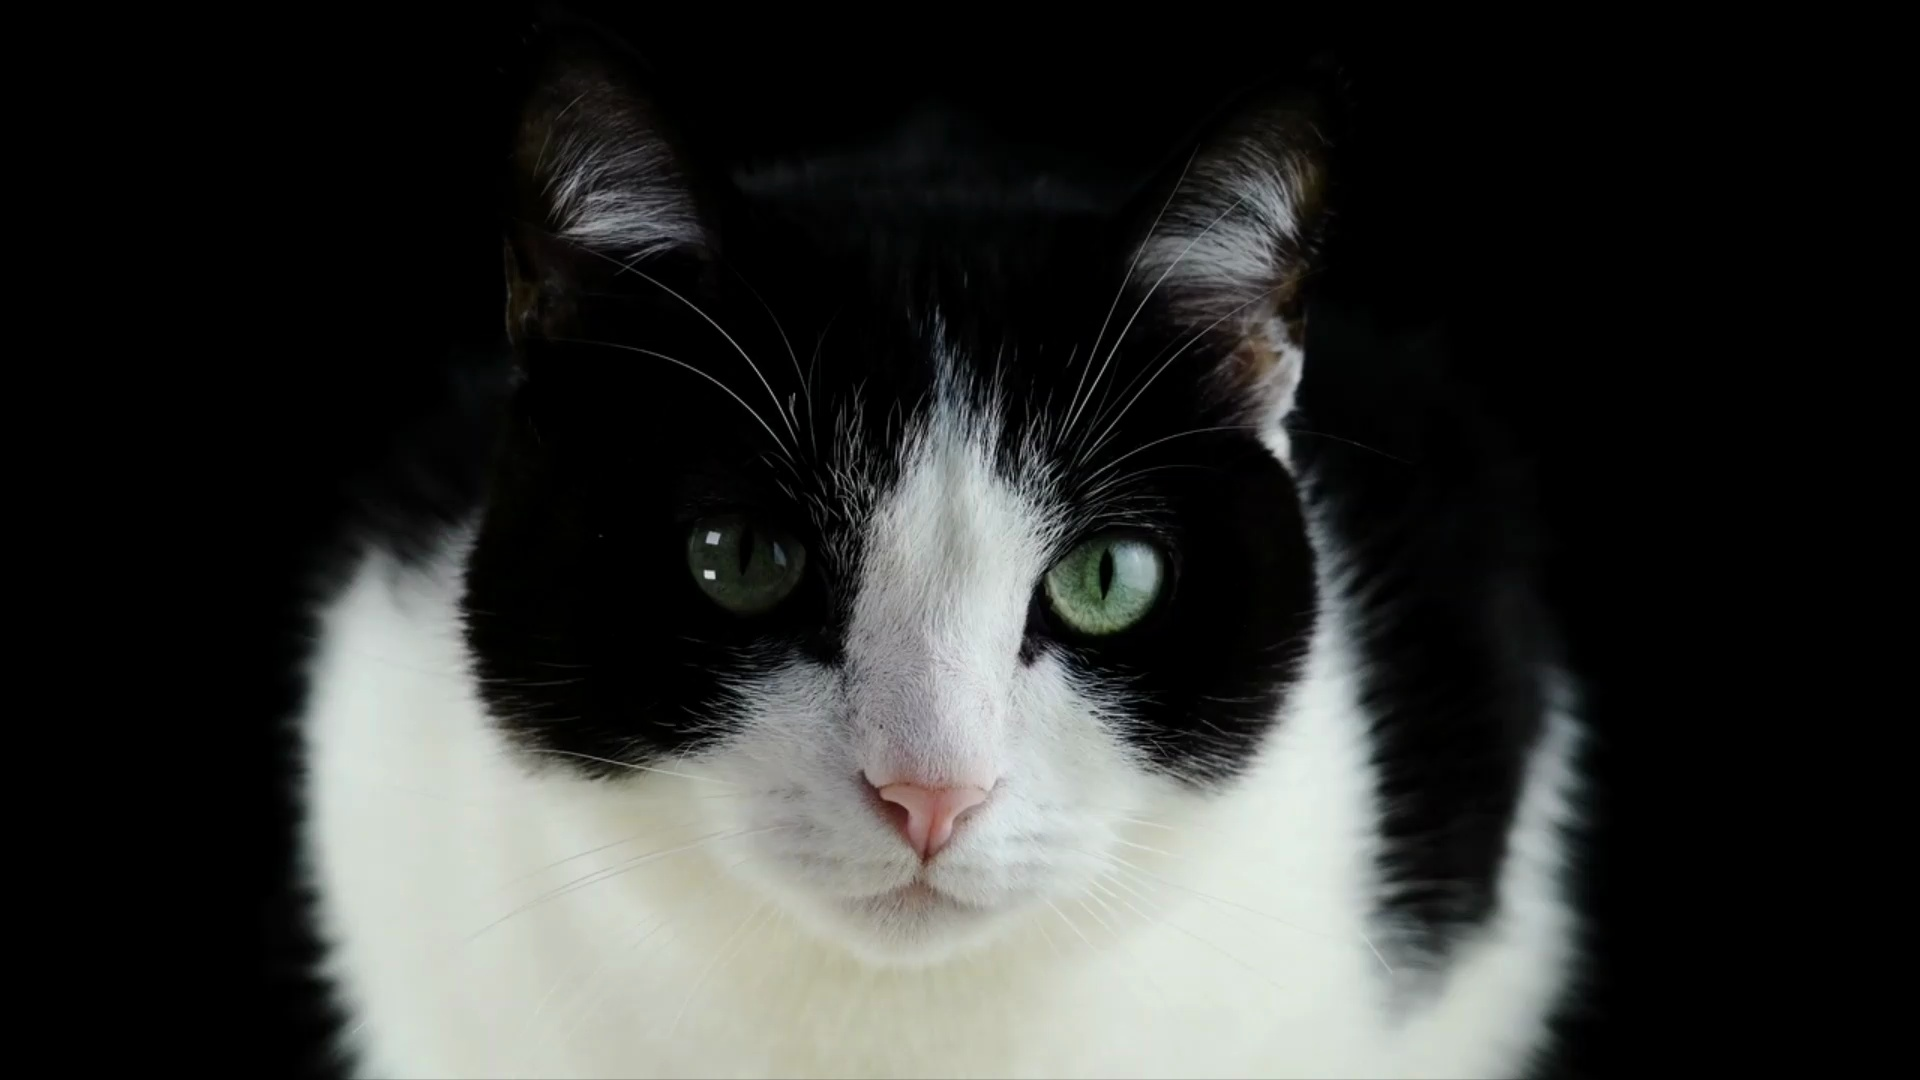
\includegraphics[width=0.42\linewidth]{../dataset/images/output/6324034_boundary_frame78.jpg} \\
フレーム 77 & フレーム 78 \\
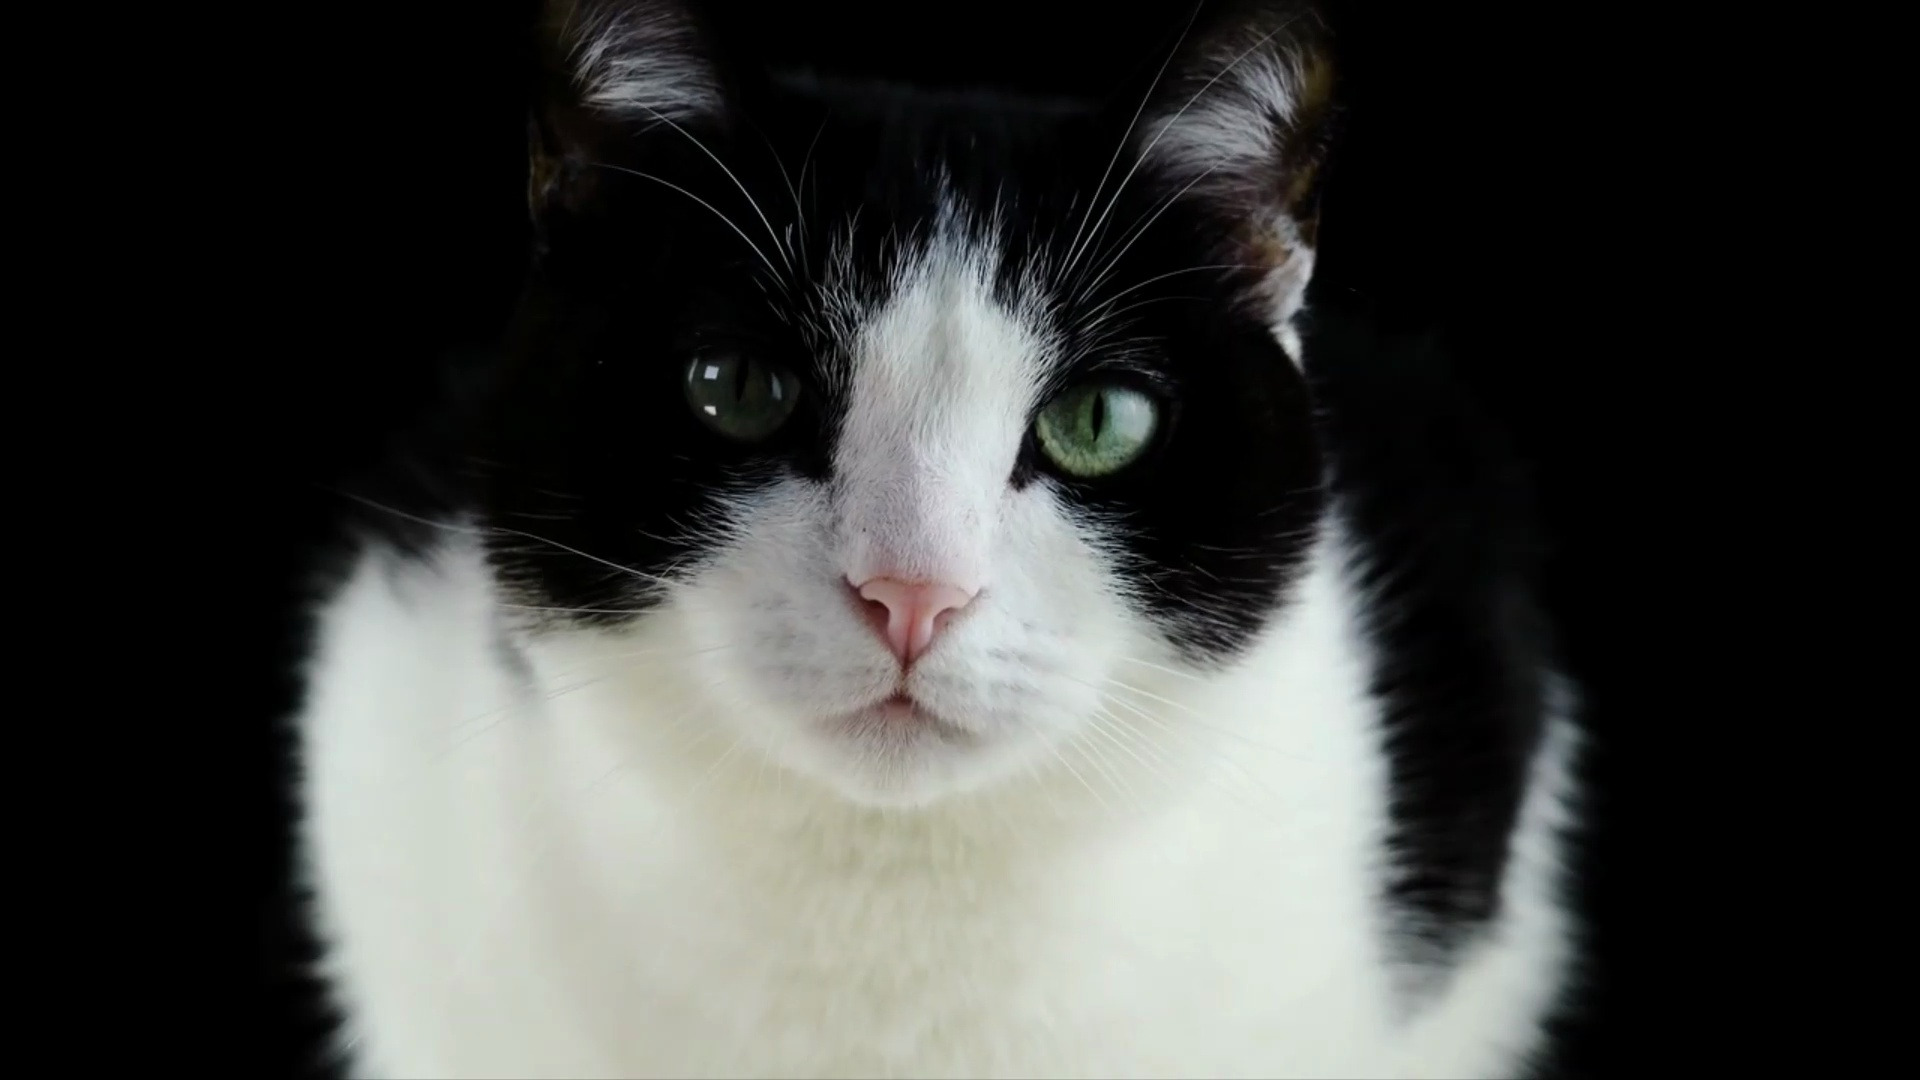
\includegraphics[width=0.42\linewidth]{../dataset/images/output/6324034_boundary_frame213.jpg} &
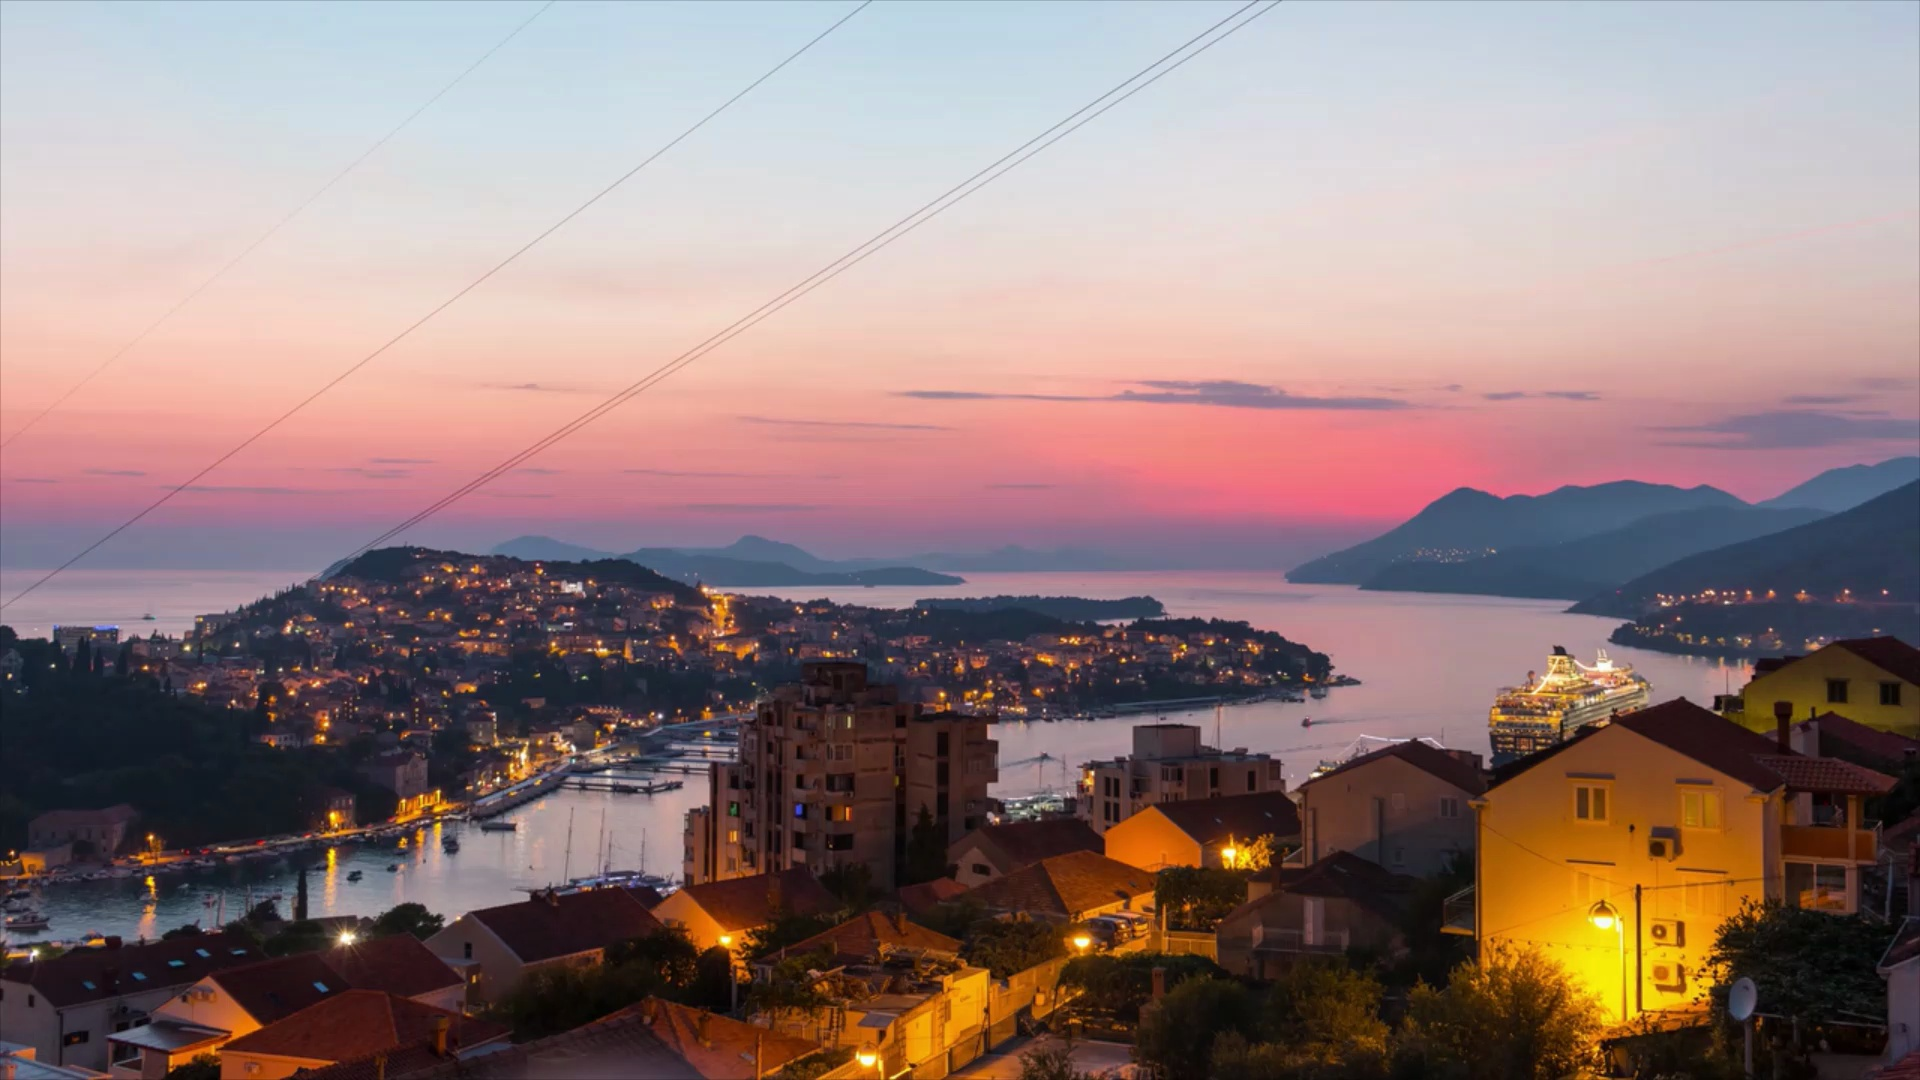
\includegraphics[width=0.42\linewidth]{../dataset/images/output/6324034_boundary_frame214.jpg} \\
フレーム 213 & フレーム 214 \\
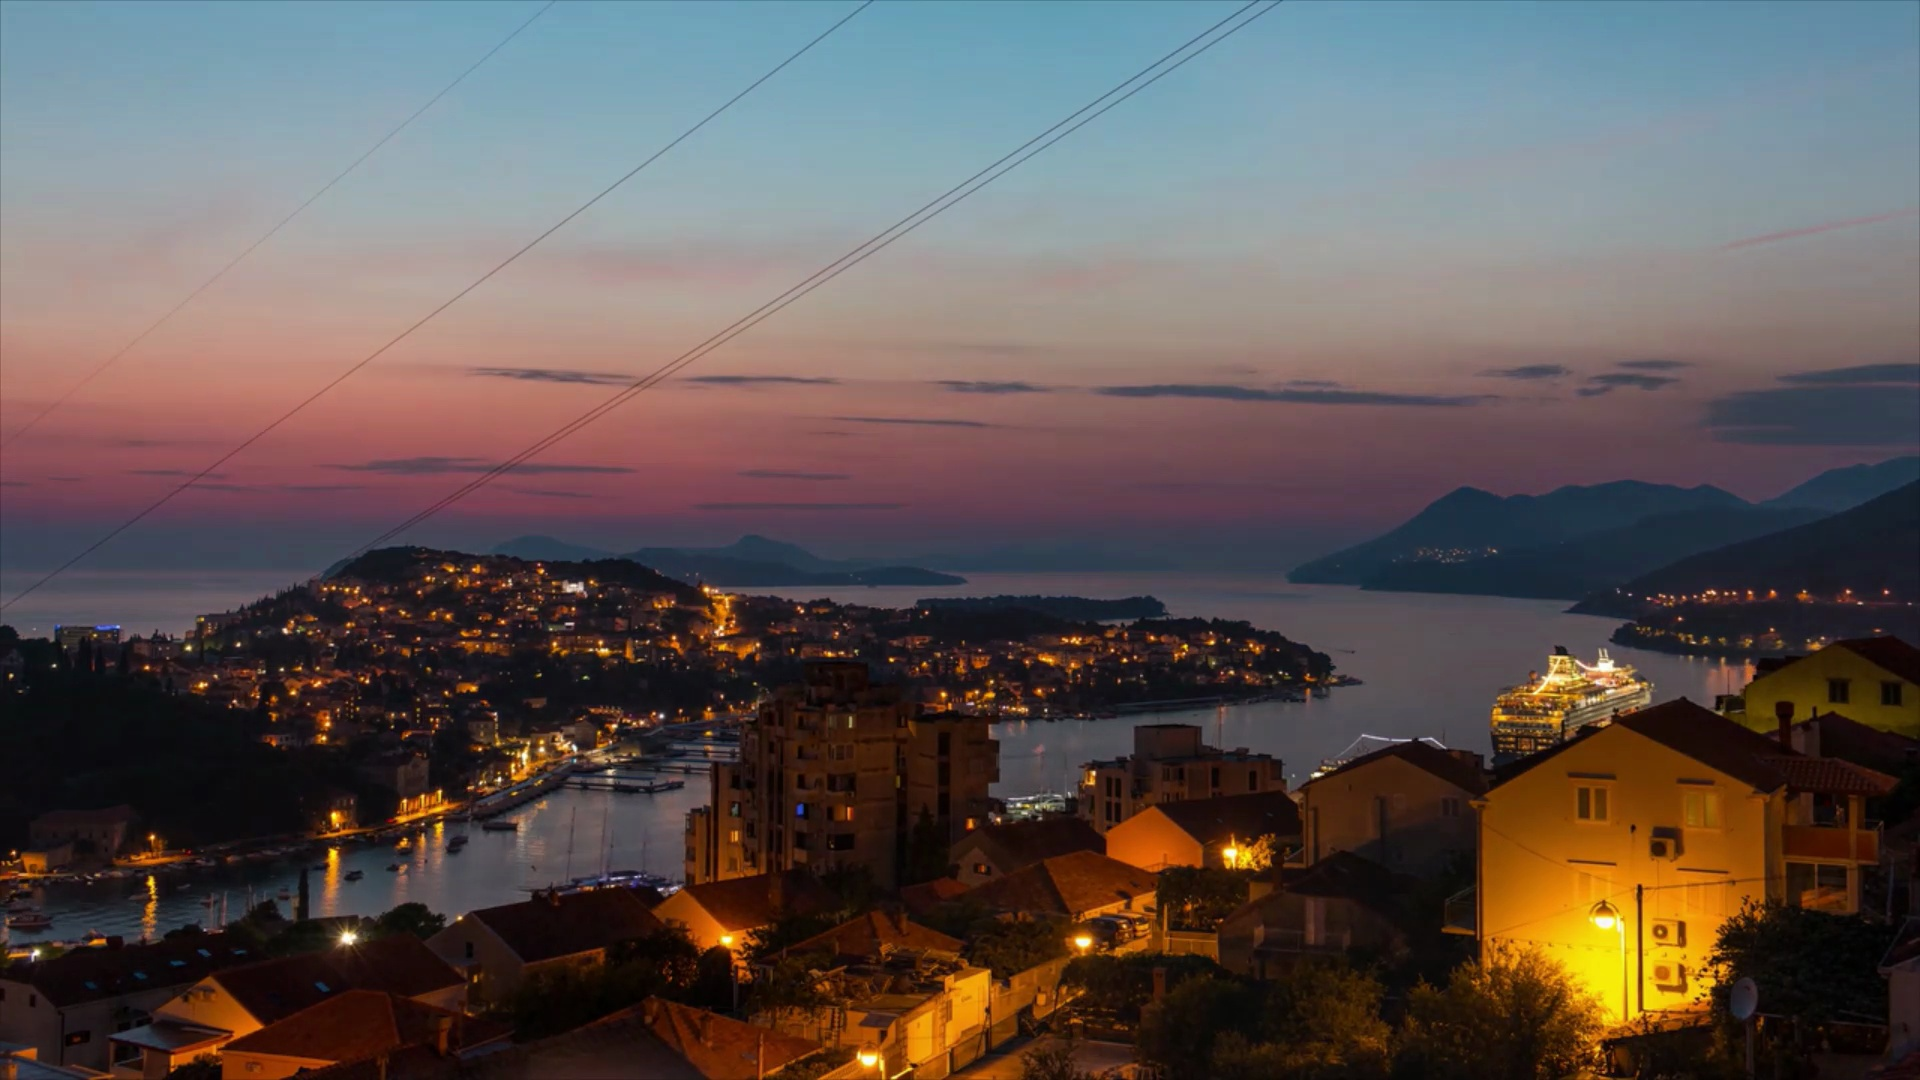
\includegraphics[width=0.42\linewidth]{../dataset/images/output/6324034_boundary_frame256.jpg} &
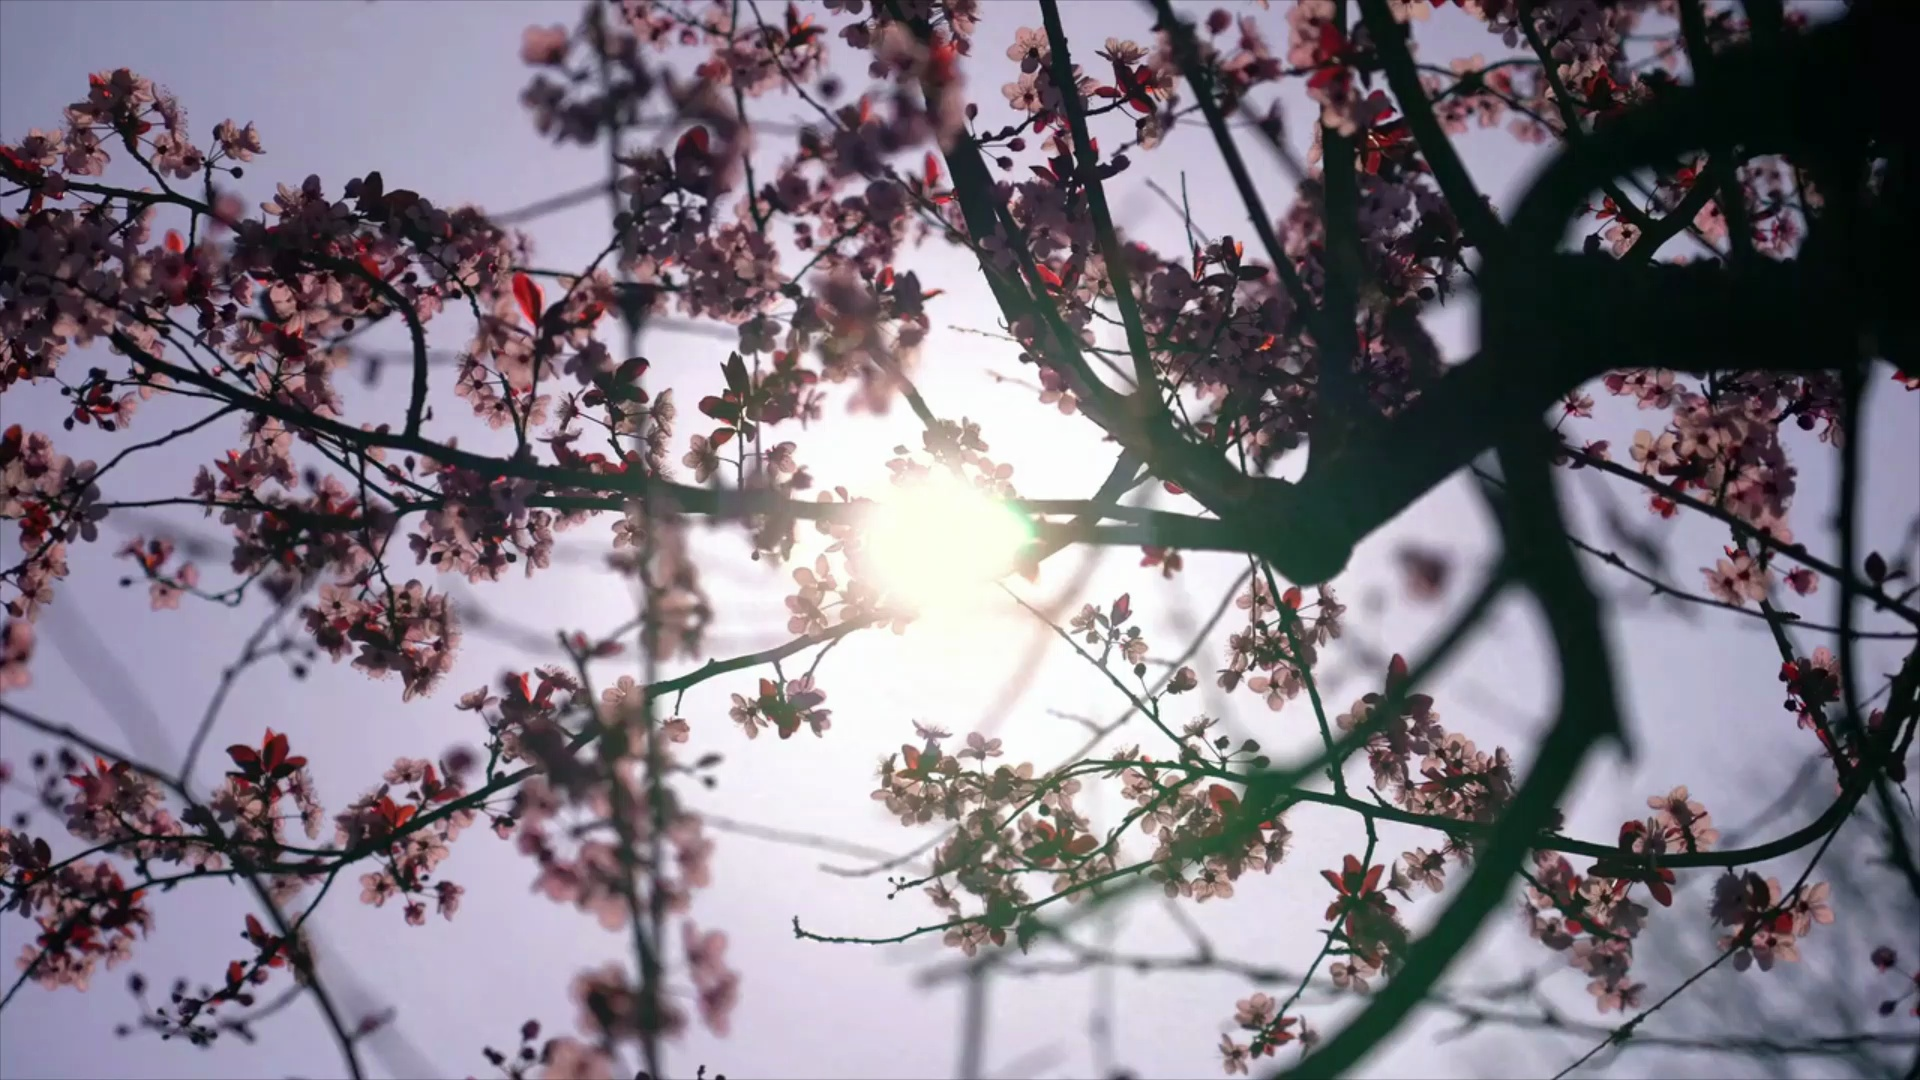
\includegraphics[width=0.42\linewidth]{../dataset/images/output/6324034_boundary_frame257.jpg} \\
フレーム 256 & フレーム 257 \\
\end{tabular}
\caption{検出された変わり目(右列)とその直前フレーム(左列)}
\label{fig:boundary}
\end{figure}

\subsection{課題 8: Video クラスの動作確認}

People - 84973.mp4 で Video クラスをインスタンス化し、{\tt parse\_filename}、
{\tt create\_thumbnail}、{\tt get\_info} が正しく動作すること
(title: People、video\_id: 84973、thumbnail: フレーム 185、形状 (720, 1280, 3))を
確認した。また、高階関数方式の {\tt process\_video} に二値化・グレースケール化・
色反転の 3 関数をそれぞれ渡し、3 本の処理済み動画が生成されることを確認した。
このうち色反転を渡した結果は課題 4 の出力と同一の処理である。

以上より、作成したプログラムは 8 つの課題すべてを満たして正しく動作している。
詳細な検討は次節の考察で行う。
